To determine whether our \textbf{multi-modal} approach outperformed a traditional \textbf{vision only} approach, we measured the average number of robot guesses and human guesses in games played with each fold of objects.
The systems were identical in fold 0 since both were untrained.
In the end, we trained the systems on all available data to calculate predicate classifier agreement with human labels.

\begin{figure}
\centering
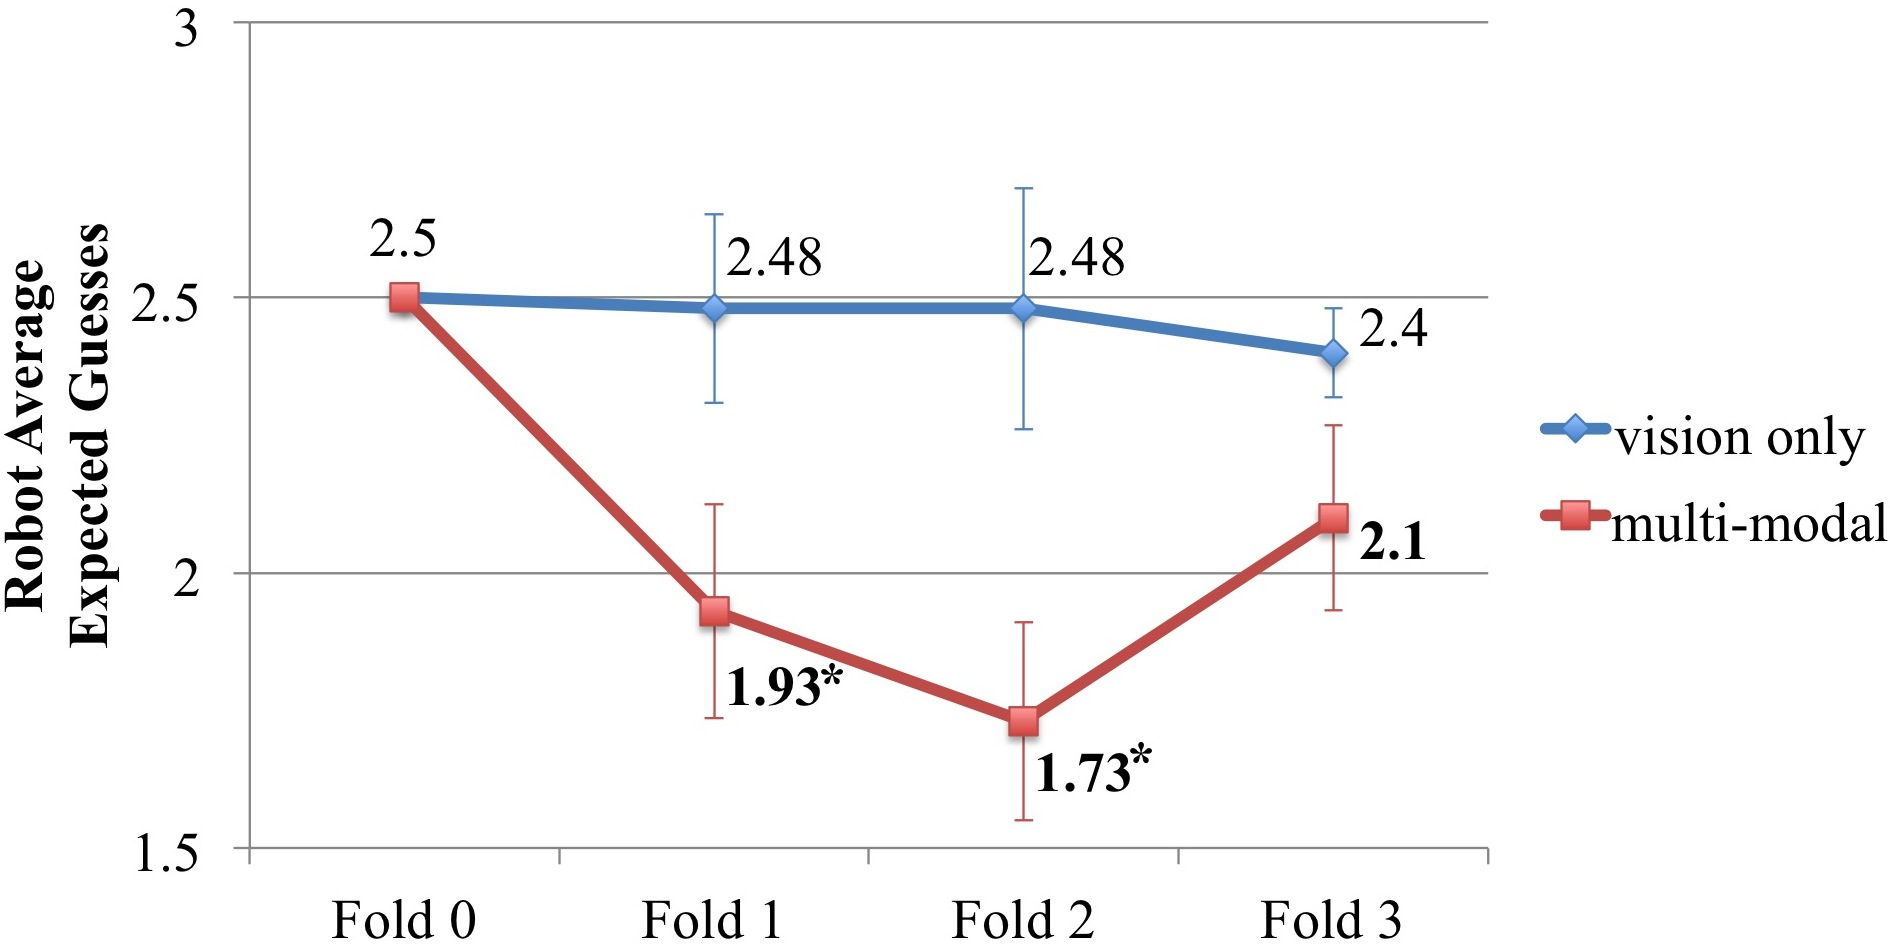
\includegraphics[width=0.5\textwidth]{figures/robot_guesses_error_bars.jpg}
\caption{Average expected number of guesses the robot made on each human turn with standard error bars shown.
\textbf{Bold}: significantly lower than the average at fold 0 with $p<0.05$ (unpaired Student's $t$-test).
\textbf{*}: significantly lower than the competing system on this fold on participant-by-participant basis with $p<0.05$ (paired Student's $t$-test).}
\label{fig:robot_guesses}
\end{figure}

\textbf{Robot guess.} Figure~\ref{fig:robot_guesses} shows the average number of robot guesses for the games in each fold. Because we had access to the scores the robot assigned each object, we calculated the {\it expected} number of robot guesses for each turn.
For example, if all 4 objects were tied for first, the expected number of robot guesses for that turn was 2.5, regardless of whether it got (un)lucky and picked the correct object (last)first.\footnote{2.5 is the expected number for 4 tied objects because the probability of picking in any order is equal, so the expected turn to get the correct object is $\frac{1+2+3+4}{4} = \frac{10}{4} = 2.5$}

After training on just one fold, our \textbf{multi-modal} approach performs statistically significantly better than the expected number of turns for guessing (the strategy for the untrained fold 0 system) for the remainder of the games.
The \textbf{vision only} system, by contrast, is never able to differentiate itself significantly from random guessing, even as more training data becomes available.
We suspect the number of objects is too small for the \textbf{vision only} system to develop decent models of many predicates, whereas \textbf{multi-modal} exploration allows that system to extract more information per object.

\textbf{Human guess.} Neither the \textbf{vision only} nor \textbf{multi-modal} system's performance improves on this metric with statistical significance as more training data is seen.
Human guesses hovered around 2.5 throughout all levels of training and sets of objects.

This result highlights the difficulty of the robot's turn in an \ispy framework, which requires not just good coverage of grounded words (as when figuring out what object the human is describing), but also high accuracy when using classifiers on new objects.
Context classifiers which had few examples could achieve confidence $\kappa=1$, making the predicates they represented more likely to be chosen to describe objects.
It is possible that the system would have performed better on this metric if the predicate scoring function $R$ additionally favored predicates with many examples.

\textbf{Predicate Agreement.} After training the predicate classifiers using data gathered over all folds of objects, we calculated the precision, recall, $F_1$, and $\kappa$ scores of each against the human labels on which they were trained.
Table~\ref{tab:predicate_results} gives these metrics for the 54 predicates shared between the systems.\footnote{There were 129 predicates total between both systems.
The results in Table~\ref{tab:predicate_results} hold with significance for an unsigned $t$-test across all 129 predicates as well, with the exception of $\kappa$ differing with only $p<0.1$.}

\begin{table}
\centering
\begin{tabular}[h]{|l|r|r|}
	\hline
	\bf Metric & \multicolumn{2}{c|}{\bf System} \\ \hline \hline
	& \bf vision only & \bf multi-modal \\ \hline
	precision & .306 & .497\textbf{*} \\
	recall & .340 & .530\textbf{*} \\
	\bf $F_1$ & .317 & .498\textbf{*} \\
	\bf $\kappa$ & .105 & .212\textbf{*} \\ \hline
\end{tabular}
\caption{Agreement metrics of predicate classifiers shared between the \textbf{vision only} and \textbf{multi-modal} systems.
\textbf{*}: a significantly greater than competing system with $p<0.05$ (Student's paired $t$-test).}
\label{tab:predicate_results}
\end{table}

Across the objects our robot explored, our \textbf{multi-modal} system achieves consistently better agreement with human assignments of predicates to objects than does the \textbf{vision only} system.
